\documentclass[10pt]{article}
\usepackage[polish]{babel}
\usepackage[utf8]{inputenc}
\usepackage[T1]{fontenc}
\usepackage{amsmath}
\usepackage{amsfonts}
\usepackage{amssymb}
\usepackage[version=4]{mhchem}
\usepackage{stmaryrd}
\usepackage{graphicx}
\usepackage[export]{adjustbox}
\graphicspath{ {./images/} }

\title{OD SZKOLNIAKA DO ŻAKA }

\author{}
\date{}


\begin{document}
\maketitle
klasy 5 i 6 szkoły podstawowej\\
rok szkolny 2020/2021

\section*{Zadania - etap III}
Zadanie 1. Suma pięciu kolejnych liczb naturalnych jest równa 1500. Ile wynosi największa z tych liczb?

Zadanie 2. Wiadomo, że trójkąt ABC ma obwód 37 cm . Na boku BC wyznaczono punkt M taki, że kąty CAM i ACM mają równe miary. Wiadomo też, że trójkąt ABM ma obwód równy 24 cm . Oblicz długość boku AC.

Zadanie 3. W trójkącie ostrokątnym \(A B C\) zaznaczono kąty między bokiem AC tego trójkąta a wysokościami wyprowadzonymi z wierzchołków A i C. Kąty te mają odpowiednio miary \(20^{\circ}\) i \(40^{\circ}\). Oblicz miary kątów trójkąta ABC.\\
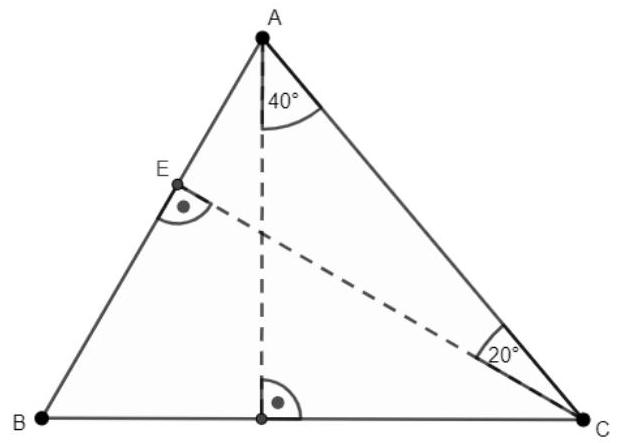
\includegraphics[max width=\textwidth, center]{2024_11_21_9046c7087d49c1f0c0e5g-1}

Zadanie 4. Porównaj liczby: \(a=\frac{1}{100} \cdot \frac{2}{99} \cdot \frac{3}{98} \cdot \ldots \cdot \frac{99}{2} \cdot \frac{100}{1}\) oraz \(b=\frac{1}{1 \cdot 2}+\frac{1}{2 \cdot 3}+\frac{1}{3 \cdot 4}+\ldots+\frac{1}{18 \cdot 19}+\frac{1}{19 \cdot 20}\).

Zadanie 5. W prostokącie \(A B C D\) bok \(A D\) stanowi \(\frac{3}{8}\) boku \(A B\). Z wierzchołka D poprowadzono odcinek do punktu \(M\), będącego środkiem boku \(A B\). Odcinek ten podzielił prostokąt ABCD na dwie figury: trapez o obwodzie 20 cm i trójkąt o obwodzie równym 12 cm . Oblicz długości boków tego prostokąta.


\end{document}